\documentclass[11pt]{article}
\usepackage[margin=1in]{geometry}
\usepackage{amsmath,amssymb,amsthm,mathtools}
\usepackage{graphicx}
\usepackage{microtype}
\usepackage[hidelinks]{hyperref}

\newtheorem{theorem}{Theorem}
\newtheorem{lemma}{Lemma}
\newcommand{\C}{\mathbb C}
\newcommand{\Z}{\mathbb Z}
\newcommand{\wind}{\operatorname{wind}}

\title{Increasing second quotients and asymptotically real zeros}
\author{Candidate full proof of the conjecture in arXiv:2008.04754}
\date{11 August 2026}

\begin{document}
\maketitle

\begin{center}
\fbox{\parbox{0.91\textwidth}{
\textbf{Status: candidate full proof, likely valid.}
If a real entire function has positive Taylor coefficients and
$1<q_2\leq q_3\leq\cdots$ for its second coefficient quotients, then
all but finitely many of its zeros are real and simple.  This proves the
source's explicit conjecture and removes its lower bound
$q_2\geq2\sqrt[3]{2}$.}}
\end{center}

\section{Source conjecture}

The source is T.~H.~Nguyen and A.~Vishnyakova,
\emph{On the entire functions from the Laguerre--P\'olya I class having
the increasing second quotients of Taylor coefficients},
arXiv:2008.04754, published in \emph{J. Math. Anal. Appl.} 498 (2021),
124959 \cite{NV}.

For
\[
 f(z)=\sum_{k=0}^{\infty}a_kz^k,\qquad a_k>0,
\]
define
\[
 q_n=\frac{a_{n-1}^2}{a_{n-2}a_n}\qquad(n\geq2).
\]
The source proves that all but finitely many zeros are real and simple when
$2\sqrt[3]{2}\leq q_2\leq q_3\leq\cdots$.  It then conjectures the same
conclusion under the qualitative assumption
$1<q_2\leq q_3\leq\cdots$.

\begin{figure}[ht]
\centering
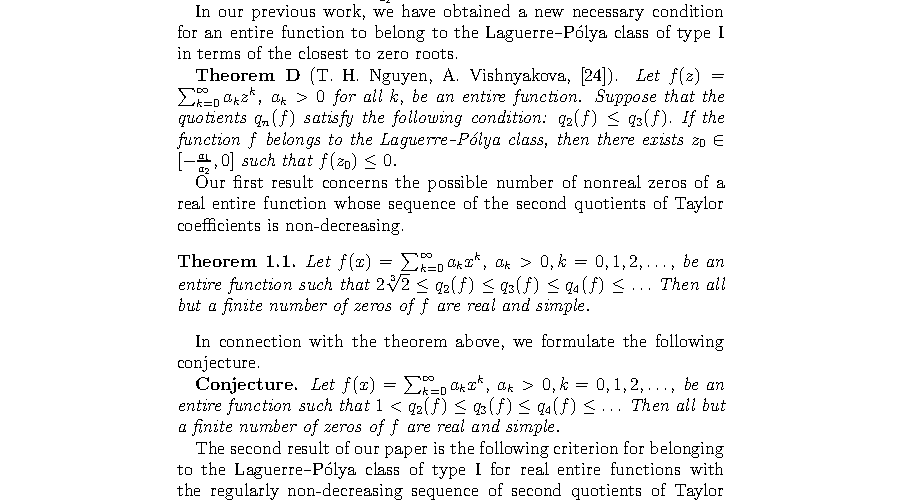
\includegraphics[width=\textwidth]{figures/conjecture_page5.png}
\caption{Theorem~1.1 and the explicit conjecture on page 5 of the source.}
\label{fig:conjecture}
\end{figure}

\section{Proof intuition}
Rescale at the $n$th coefficient peak.  Monotonicity of the second quotients
makes the normalized Laurent tails uniformly summable, while the rescaled
functions converge either to a Jacobi triple-product with simple positive
geometric zeros or to $1-z^{-1}$.  Rouch\'e's theorem then produces one
simple real zero near every large coefficient scale.  A fixed-circle
argument-principle count shows that only finitely many zeros are left over,
so the produced zeros exhaust the tail of the zero set.

\section{Coefficient-peak scaling}

Multiplying the function and rescaling its variable by positive constants
does not change its second quotients or the reality and simplicity of its
zeros.  We may therefore assume $a_0=a_1=1$.  Put
\[
 p_n=\frac{a_{n-1}}{a_n}\quad(n\geq1).
\]
Then $p_1=1$, $p_n/p_{n-1}=q_n$, and hence
\begin{equation}\label{eq:pn}
 p_n=q_2q_3\cdots q_n.
\end{equation}
Let
\[
 \varphi(z)=f(-z)=\sum_{k=0}^{\infty}(-1)^ka_kz^k
\]
and define, for $z\ne0$,
\begin{equation}\label{eq:Gn}
 G_n(z)=\frac{(-1)^n\varphi(p_nz)}{a_np_n^nz^n}.
\end{equation}

\begin{lemma}[Scaling limits]\label{lem:limit}
The monotone sequence $(q_n)$ has a limit $a\in[q_2,\infty]$.  The following local-uniform
limits hold on $\C\setminus\{0\}$.

If $a<\infty$, then
\begin{equation}\label{eq:Ga}
 G_n(z)\longrightarrow
 G_a(z):=\sum_{m\in\Z}(-1)^m a^{-m(m+1)/2}z^m.
\end{equation}
If $a=\infty$, then
\begin{equation}\label{eq:Ginf}
 G_n(z)\longrightarrow G_\infty(z):=1-z^{-1}.
\end{equation}
\end{lemma}

\begin{proof}
Expanding \eqref{eq:Gn} around its central coefficient gives
\[
 G_n(z)=\sum_{m=-n}^{\infty}(-1)^m c_{n,m}z^m,
\]
where
\begin{align}
 c_{n,m}&=p_n^m\frac{a_{n+m}}{a_n}
 =\prod_{j=1}^{m}\frac{p_n}{p_{n+j}} &&(m\geq0),\label{eq:cplus}\\
 c_{n,-r}&=p_n^{-r}\frac{a_{n-r}}{a_n}
 =\prod_{j=0}^{r-1}\frac{p_{n-j}}{p_n} &&(1\leq r\leq n).
 \label{eq:cminus}
\end{align}
Here empty products equal one.  Set $c=q_2>1$.  From
$p_{k}/p_{k-1}=q_k\geq c$ we obtain the uniform bounds
\begin{equation}\label{eq:bounds}
 0<c_{n,m}\leq c^{-m(m+1)/2},\qquad
 0<c_{n,-r}\leq c^{-r(r-1)/2}.
\end{equation}
On every compact annulus $\delta\leq|z|\leq R$, the corresponding two
Gaussian-type series are summable.  Thus \eqref{eq:bounds} supplies a
Weierstrass majorant for both Laurent tails.

If $q_n\to a<\infty$, formulas \eqref{eq:cplus}--\eqref{eq:cminus}
give, for every fixed $m\in\Z$,
\[
 c_{n,m}\longrightarrow a^{-m(m+1)/2}.
\]
Dominated convergence for the Laurent series proves \eqref{eq:Ga}.  If
$q_n\to\infty$, only $c_{n,0}=c_{n,-1}=1$ survive; every other fixed
coefficient tends to zero.  The same majorants prove \eqref{eq:Ginf}.
\end{proof}

For finite $a$, put $q=a^{-1}\in(0,1)$.  The Jacobi triple-product
identity gives
\begin{equation}\label{eq:triple}
 G_a(z)=(qz;q)_\infty(1/z;q)_\infty(q;q)_\infty,
\end{equation}
where $(x;q)_\infty=\prod_{j=0}^{\infty}(1-xq^j)$.  Consequently the
zeros of $G_a$ are precisely
\begin{equation}\label{eq:limitzeros}
 \{a^k:k\in\Z\},
\end{equation}
and every one is positive and simple.  The limit $G_\infty=1-z^{-1}$
likewise has the single simple zero $1$ on $\C\setminus\{0\}$.

\section{Proof of the conjecture}

\begin{theorem}\label{thm:main}
Let $f(z)=\sum_{k=0}^{\infty}a_kz^k$ be entire, with $a_k>0$, and suppose
\[
 1<q_2\leq q_3\leq q_4\leq\cdots.
\]
Then all but finitely many zeros of $f$ are real, negative, and simple.
\end{theorem}

\begin{proof}
We use the preceding normalization.  First suppose $q_n\to a<\infty$.
Choose $\varepsilon>0$ so small that the closed disk
\[
 D=\{z:|z-1|\leq\varepsilon\}
\]
contains no zero of $G_a$ except $1$, and also
\begin{equation}\label{eq:eps}
 1+\varepsilon<\sqrt a,
 \qquad
 \frac{1+\varepsilon}{1-\varepsilon}<a.
\end{equation}
Lemma~\ref{lem:limit} and Rouch\'e's theorem imply that, for every
sufficiently large $n$, $G_n$ has exactly one zero in $D$, counted with
multiplicity.  Since $G_n$ is real on the real axis and $D$ is invariant
under conjugation, that unique zero is real; it is simple and belongs to
$(1-\varepsilon,1+\varepsilon)$.  By \eqref{eq:Gn}, $\varphi$ therefore
has a simple positive zero
\begin{equation}\label{eq:xn}
 x_n\in\bigl((1-\varepsilon)p_n,(1+\varepsilon)p_n\bigr).
\end{equation}
The second inequality in \eqref{eq:eps} and $q_{n+1}\to a$ show that
these intervals are pairwise disjoint once $n$ is large enough.

It remains to show that these zeros account for all but finitely many zeros.
Set $r=\sqrt a$.  By \eqref{eq:limitzeros}, $G_a$ has no zero on
$|z|=r$.  Local-uniform convergence on that circle implies that, for all
large $n$,
\[
 \wind\bigl(G_n(r e^{it}),0\bigr)
 =\wind\bigl(G_a(r e^{it}),0\bigr)=:W,
\]
where $W$ is a fixed integer.  The meromorphic function $G_n$ has a pole
of exact order $n$ at zero, and its other zeros are exactly the rescaled
zeros of $\varphi$.  The argument principle therefore yields
\begin{equation}\label{eq:count}
 N_\varphi(rp_n)=n+W,
\end{equation}
where zeros in $|z|<rp_n$ are counted with multiplicity.

Choose $K$ large enough that all preceding assertions hold and
$K+W-1\geq0$.  For every $n\geq K$, the distinct simple positive zeros
$x_K,\ldots,x_n$ all lie in $|z|<rp_n$, by the first inequality in
\eqref{eq:eps}.  Comparing their number with \eqref{eq:count}, at most
$K+W-1$ zeros in that disk are not members of this sequence.  Since
$p_n\to\infty$, the disks exhaust the plane.  Hence globally only finitely
many zeros of $\varphi$ are not among the simple positive zeros $x_n$.

If $q_n\to\infty$, repeat the same argument with the limit
$G_\infty=1-z^{-1}$ and $r=2$.  Choose $0<\varepsilon<1$ with
$1+\varepsilon<2$.  Rouch\'e again gives one simple real zero near every
$p_n$; the corresponding intervals are eventually disjoint because
$q_{n+1}\to\infty$.  On $|z|=2$, the winding number of
$(z-1)/z$ is zero, so the analogue of \eqref{eq:count} is simply
$N_\varphi(2p_n)=n$.  The same exhaustion argument finishes this case.

Thus all but finitely many zeros of $\varphi(z)=f(-z)$ are positive real
and simple.  Equivalently, all but finitely many zeros of $f$ are negative
real and simple.
\end{proof}

\section{Scope and novelty}

The theorem proves the explicit conjecture displayed in
Figure~\ref{fig:conjecture}.  It strengthens the source's Theorem~1.1 by
removing the numerical lower bound on $q_2$.  It does not settle the
separate question of whether extra hypotheses can be removed from the
source's criterion ensuring that \emph{every} zero is real.

The local run indexes and bounded web searches on 11 August 2026 used the
arXiv identifier, exact title and conjecture, increasing second quotients,
later work by the same authors, coefficient-peak scaling, and Jacobi
triple-product terminology.  They found the source, a 2021 follow-up that
bounds the possible number of nonreal zeros, and a 2022 thesis retaining
further questions, but no proof of this conjecture and no matching scaling
argument.  Novelty confidence is moderate because coverage is bounded.

\begin{thebibliography}{9}
\bibitem{NV}
T.~H.~Nguyen and A.~Vishnyakova,
\emph{On the entire functions from the Laguerre--P\'olya I class having the
increasing second quotients of Taylor coefficients},
J. Math. Anal. Appl. 498 (2021), 124959;
arXiv:2008.04754.
\url{https://arxiv.org/abs/2008.04754}.
\end{thebibliography}

\end{document}
